\documentclass{beamer} 
\usepackage{amsmath,amsthm}
\usepackage{graphicx,microtype,parskip}
\usepackage{caption,subcaption,multirow}
\usepackage{attrib}

\frenchspacing

\usetheme{default}
\usecolortheme{whale}

\setbeamertemplate{navigation symbols}{}

\setbeamercolor{title}{fg=blue,bg=white}

\setbeamercolor{block title}{fg=white,bg=gray}
\setbeamercolor{block body}{fg=black,bg=lightgray}

\setbeamercolor{block title alerted}{fg=white,bg=darkgray}
\setbeamercolor{block body alerted}{fg=black,bg=lightgray}


\title{Confessions of a (former) denimhead}
\author{Peter D Smits}
\institute{Committee on Evolutionary Biology, University of Chicago}
\date{}

\begin{document}

\begin{frame}
  \maketitle
\end{frame}

\begin{frame}
  \includegraphics[height = \textheight, width = \textwidth, keepaspectratio = true]{figure/long}
\end{frame}

\begin{frame}
  \includegraphics[height = \textheight, width = \textwidth, keepaspectratio = true]{figure/me2}
\end{frame}

\begin{frame}
  \frametitle{Denimhead?}

  Connoiseur of fine and high end denim, frequently raw.
\end{frame}

\begin{frame}
  \frametitle{A brief history of ``serge de N\^{i}mes''}

  \begin{center}
    \includegraphics[height = 0.4\textheight, width = \textwidth, keepaspectratio = true]{figure/nimes_map}

    \includegraphics[height = 0.4\textheight, width = \textwidth, keepaspectratio = true]{figure/nimes_city}
  \end{center}
\end{frame}

\begin{frame}
  \frametitle{General approach}

  \begin{center}
    \includegraphics[height = 0.8\textheight, width = \textwidth, keepaspectratio = true]{figure/raw}
  \end{center}
\end{frame}

\begin{frame}
  \frametitle{Raw?}
  \begin{columns}
    \begin{column}{0.5\textwidth}
      \includegraphics[height = 0.8\textheight, width = \textwidth, keepaspectratio = true]{figure/dye_1}
    \end{column}
    \begin{column}{0.5\textwidth}
      \includegraphics[height = 0.4\textheight, width = \textwidth, keepaspectratio = true]{figure/dye_3}
      
      \includegraphics[height = 0.4\textheight, width = \textwidth, keepaspectratio = true]{figure/dye_4}
    \end{column}
  \end{columns}
\end{frame}

\begin{frame}
  \frametitle{Selvedge?}
  \begin{columns}
    \begin{column}{0.5\textwidth}
      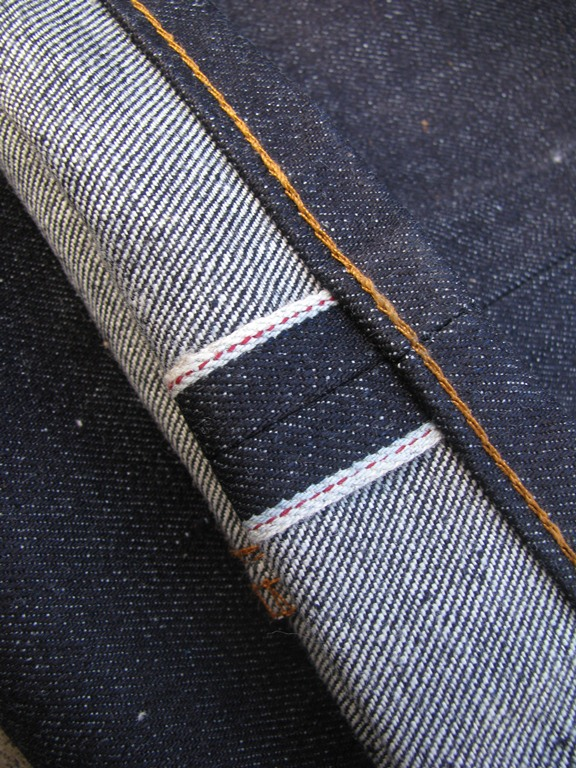
\includegraphics[height = 0.8\textheight, width = \textwidth, keepaspectratio = true]{figure/selvedge_exp}
    \end{column}
    \begin{column}{0.5\textwidth}
      \includegraphics[height = 0.8\textheight, width = \textwidth, keepaspectratio = true]{figure/selvedge_worn}
    \end{column}
  \end{columns}
\end{frame}

\begin{frame}
  \frametitle{Anatomy of a fade}

  \includegraphics[height = 0.8\textheight, width = \textwidth, keepaspectratio = true]{figure/Selvedge_WearPatterns}
\end{frame}

\begin{frame}
  \frametitle{Opinions}
  \begin{center}
    \includegraphics[height = 0.8\textheight, width = \textwidth, keepaspectratio = true]{figure/cuff_1}
    \includegraphics[height = 0.8\textheight, width = \textwidth, keepaspectratio = true]{figure/cuff_2}
    \includegraphics[height = 0.8\textheight, width = \textwidth, keepaspectratio = true]{figure/cuff_4}
  \end{center}
\end{frame}

\begin{frame}
  \frametitle{Philosophy}
  \begin{footnotesize}
    \begin{quotation}
      premium denim is pure semiotics. premium denim elitism is a codification of/for insiders. it operates on the same plane as the rest of fashion, including and excluding based on labels (read: taste). the only thing which makes it exemplary is that even poor people can gain lifetime access if they spend the ticket price for a single pair of premium denim -- ~150USD -- which they will, in turn, wear every day. if you are wearing a pair of choice premium denim -- APC, Acne being the most popular -- even if you wear 5 dollar thrift store canvas shoes and a 5 dollar t-shirt with no money left over for undies or socks, you are in the game. in this way it is a worthwhile investment if you privilege being looked and accepted at by fellow denim insiders. premium denim is the great equalizer. a person who makes no money, through association by denim will be on the same level as even the richest person who looks for the qualities in a pair of jeans as dictated by denim insiders.

      \tiny{\attrib{messageboard quote, Francoifido}}
    \end{quotation}
  \end{footnotesize}
\end{frame}

\begin{frame}
  Let's go through some brands\dots

  \vspace{3cm}

  \tiny{\attrib{with copy from denimfuture.com}}
\end{frame}

\begin{frame}
  \frametitle{APC}
  \includegraphics[height = 0.8\textheight, width = \textwidth, keepaspectratio = true]{figure/apc_guide}
\end{frame}

\begin{frame}
  \frametitle{APC}
  \includegraphics[height = 0.8\textheight, width = \textwidth, keepaspectratio = true]{figure/apc_fade}
\end{frame}

\begin{frame}
  \frametitle{Samurai}
  \includegraphics[height = 0.8\textheight, width = \textwidth, keepaspectratio = true]{figure/samurai_contest}
\end{frame}

\begin{frame}
  \frametitle{Samurai}
  \begin{columns}
    \begin{column}{0.5\textwidth}
      \includegraphics[height = 0.8\textheight, width = \textwidth, keepaspectratio = true]{figure/samurai_full}
    \end{column}
    \begin{column}{0.5\textwidth}
      \includegraphics[height = 0.4\textheight, width = \textwidth, keepaspectratio = true]{figure/samurai_age}

      \includegraphics[height = 0.4\textheight, width = \textwidth, keepaspectratio = true]{figure/samurai_fade}
    \end{column}
  \end{columns}
\end{frame}

\begin{frame}
  \frametitle{Pure Blue Japan}
  \includegraphics[height = 0.8\textheight, width = \textwidth, keepaspectratio = true]{figure/pbj_contest}
\end{frame}

\begin{frame}
  \frametitle{Pure Blue Japan}
  \begin{columns}
    \begin{column}{0.5\textwidth}
      \includegraphics[height = 0.8\textheight, width = \textwidth, keepaspectratio = true]{figure/pbj2}
    \end{column}
    \begin{column}{0.5\textwidth}
      \includegraphics[height = 0.4\textheight, width = \textwidth, keepaspectratio = true]{figure/pbjc_fade2}

      \includegraphics[height = 0.4\textheight, width = \textwidth, keepaspectratio = true]{figure/pbj_fade3}
    \end{column}
  \end{columns}
\end{frame}

\begin{frame}
  \frametitle{Flat Head}
  \includegraphics[height = 0.8\textheight, width = \textwidth, keepaspectratio = true]{figure/flathead_contest}
\end{frame}

\begin{frame}
  \frametitle{Flat Head}
  \begin{columns}
    \begin{column}{0.5\textwidth}
      \includegraphics[height = 0.4\textheight, width = \textwidth, keepaspectratio = true]{figure/flat_head1}

      \includegraphics[height = 0.4\textheight, width = \textwidth, keepaspectratio = true]{figure/flat_head2}
    \end{column}
    \begin{column}{0.5\textwidth}
      \includegraphics[height = 0.8\textheight, width = \textwidth, keepaspectratio = true]{figure/flat_head_jacket}
    \end{column}
  \end{columns}
\end{frame}

\begin{frame}
  \frametitle{Eternal}
  \includegraphics[height = 0.8\textheight, width = \textwidth, keepaspectratio = true]{figure/eternal_contest}
\end{frame}

\begin{frame}
  \frametitle{Eternal}
  \begin{columns}
    \begin{column}{0.5\textwidth}
      \includegraphics[height = 0.8\textheight, width = \textwidth, keepaspectratio = true]{figure/eternal_4}
    \end{column}
    \begin{column}{0.5\textwidth}
      \includegraphics[height = 0.4\textheight, width = \textwidth, keepaspectratio = true]{figure/eternal_1}

      \includegraphics[height = 0.4\textheight, width = \textwidth, keepaspectratio = true]{figure/eternal_3}
    \end{column}
  \end{columns}
\end{frame}

\begin{frame}
  \frametitle{Momotaro}
  \begin{columns}
    \begin{column}{0.5\textwidth}
      \includegraphics[height = 0.8\textheight, width = \textwidth, keepaspectratio = true]{figure/momo_full}
    \end{column}
    \begin{column}{0.5\textwidth}
      \includegraphics[height = 0.8\textheight, width = \textwidth, keepaspectratio = true]{figure/momo_front}
    \end{column}
  \end{columns}
\end{frame}


\begin{frame}
  What about women's jeans?
\end{frame}

\begin{frame}
  \frametitle{APC}
  \begin{center}
    \includegraphics[height = 0.8\textheight, width = \textwidth, keepaspectratio = true]{figure/apc_1}
  \end{center}
\end{frame}

\begin{frame}
  \frametitle{Samurai and Flat Head}
  \begin{columns}
    \begin{column}{0.5\textwidth}
      \includegraphics[height = 0.8\textheight, width = \textwidth, keepaspectratio = true]{figure/women_3}
    \end{column}
    \begin{column}{0.5\textwidth}
      \includegraphics[height = 0.8\textheight, width = \textwidth, keepaspectratio = true]{figure/women_5}
    \end{column}
  \end{columns}
\end{frame}

\begin{frame}
  \frametitle{Momotaro}
  \begin{columns}
    \begin{column}{0.5\textwidth}
      \includegraphics[height = 0.8\textheight, width = \textwidth, keepaspectratio = true]{figure/mai_2}
    \end{column}
    \begin{column}{0.5\textwidth}
      \includegraphics[height = 0.4\textheight, width = \textwidth, keepaspectratio = true]{figure/mai_1}

      \includegraphics[height = 0.4\textheight, width = \textwidth, keepaspectratio = true]{figure/mai_4}
    \end{column}
  \end{columns}
\end{frame}

\begin{frame}
  \frametitle{Tellason}
  \begin{columns}
    \begin{column}{0.5\textwidth}
      \includegraphics[height = 0.8\textheight, width = \textwidth, keepaspectratio = true]{figure/bird_2}
    \end{column}
    \begin{column}{0.5\textwidth}
      \includegraphics[height = 0.8\textheight, width = \textwidth, keepaspectratio = true]{figure/bird_1}
    \end{column}
  \end{columns}
\end{frame}

\begin{frame}
  \frametitle{Sling and Stones}
  \begin{columns}
    \begin{column}{0.5\textwidth}
      \includegraphics[height = 0.8\textheight, width = \textwidth, keepaspectratio = true]{figure/women_2}
    \end{column}
    \begin{column}{0.5\textwidth}
      \includegraphics[height = 0.8\textheight, width = \textwidth, keepaspectratio = true]{figure/women_4}
    \end{column}
  \end{columns}
\end{frame}

\begin{frame}
  \frametitle{Requiem for a denimhead}

  \begin{center}
    \includegraphics[height = 0.8\textheight, width = \textwidth, keepaspectratio = true]{figure/momo_poem}

    \tiny{\attrib{Fuckyeah Menswear}}
  \end{center}
\end{frame}

\end{document}
